\documentclass{article}
\usepackage{graphicx} % Required for inserting images
\usepackage{authblk}

\title{Classifying the Age and Sex of Rock Ptarmigans in Iceland with Convolutional Neural Networks}
\author{Brian Lin}
\affil{Institute for Computing in Research}
\date{July 2026}


\begin{document}
% Customizing bibliography heading

  
\maketitle

\begin{abstract}
Rock Ptarmigans are an important part of Icelandic culture, and as a result, their populations are monitored every year. However, the process of classifying and analyzing these birds requires upward of two months of time. This project presents a pipeline that involves using YOLOv26 on photos taken of Rock Ptarmigans in the wild to crop and standardize each photo, before feeding these images into an EfficientNetb2 model to classify each bird by age and sex. On a test set of roughly 300 photos, the model achieved an accuracy of 
nearly 70\%, an accuracy significantly higher than random guessing (25\%), suggesting that, if refined, this method of classifying Rock Ptarmigans could potentially be used to help researchers manually classify these birds.
\end{abstract}


\section{Introduction}
The Rock Ptarmigan is a medium sized bird in the Grouse tribe. They are very common in Iceland and are well known for their drastic plumage changes across the seasons. Along with being a keystone species in Iceland's ecosystem, Rock Ptarmigans are also very important to Icelandic Culture. The Rock Ptarmigan is the number one game bird in Iceland, and is also a part of many traditions, being commonly eaten as the main course for Christmas dinner. As a result, when Rock Ptarmigan populations began to decline due to overhunting in 2005, the Icelandic government restricted hunting Rock Ptarmigans for personal use, and the Icelandic Institute of Natural History began collecting population data on the birds annually. However, this process of taking photos and analyzing them is very time consuming: Photographing the population takes roughly 30 days, and manually going through each photo to determine population statistics such as age and sex takes another 30 to 50 days. In this paper, we apply transfer learning to the EfficientNetb2 model, training it on a dataset of Rock Ptarmigans in order to classify then by their age and sex. 

\section{Methodology}
\subsection{Dataset}
In order to train and test the model, we used a custom dataset consisting of 3000 images of Rock Ptarmigans taken in the wild by researchers. Due to the limited amount of data, the dataset was split 76/12/12 into training, validation, and test sets. Each image came with annotations on the age (juvenile or adult) and sex (male or female) of the birds in the pictures.

\subsection{Preprocessing}
Before we began training, each image went through multiple preprocessing steps. First, each photo was fed through the YOLOv26 \cite{sapkota2026yolo26keyarchitecturalenhancements} model to obtain a bounding box around each bird. With this, we cropped each image around the bounding boxes and added 20 pixels of safety margin on each side to ensure no parts of the bird were accidentally cropped out. Images with multiple birds in them were excluded because the annotations didn't allow for differentiation between the birds. Afterwards, each image was padded with a black border and resized to 260 by 260 pixels. Finally, data augmentation was applied to the training set: images were flipped horizontally , vertically, and rotated randomly 
to increase the diversity of the data and reduce overfitting during training.

\subsection{Model}
We used the EfficientNetb2 \cite{DBLP:journals/corr/abs-1905-11946} model with the default EfficientNetb2 weights as a base model for our training. This model was chosen due to its high top1 accuracy of 80\% on the ImageNet dataset without needing the computational demands of models such as EfficientNetb6 and ConvNeXt. 

\subsection{Training}
The model was trained over a period of 35 epochs. For training, we used an 8-bit AdamW \cite{DBLP:journals/corr/abs-1711-05101} optimizer, a cosine annealer as our learning rate scheduler, and a weight decay of 0.0001, dropout rate of 0.5, and batch size of 16 for our hyperparameters. During the first 10 epochs, the backbone of the model was frozen and the classifier head was replaced with a dropout and linear layer which was then trained with an initial learning rate of 0.001. For the remaining 25 layers, the backbone of the model was unfrozen and the entire model was fine tuned with a lower learning rate of 0.0001 to avoid catastrophic interference. The model is evaluated on the validation set after every epoch and on the test set once after training is complete. 


\section{Results}
After the end of training, the model achieved an accuracy of 69.71\% on the test set, an accuracy of 68.75\% on the validation set, and an accuracy of 95.7\% on the training set as shown in Figure 1. The large gap in accuracy between the training and valdiation/test accuracies show that the model is severely overfitting to the training data. This can further be seen in Figure 2 and Figure 3, which shows the training and validation accuracy over epochs, and training and validation loss over epochs respectively. Both figures show that the validation accuracy and loss diverge around the 12 epoch mark, signaling that the model started overfitting shortly after unfreezing the model backbone. However, despite the overfitting, the model's 69.71\% accuracy on the test set suggests that, with refinement, this method of classifying Rock Ptarmigans could be usable in the future.   

\begin{figure}[h!]
    \centering
    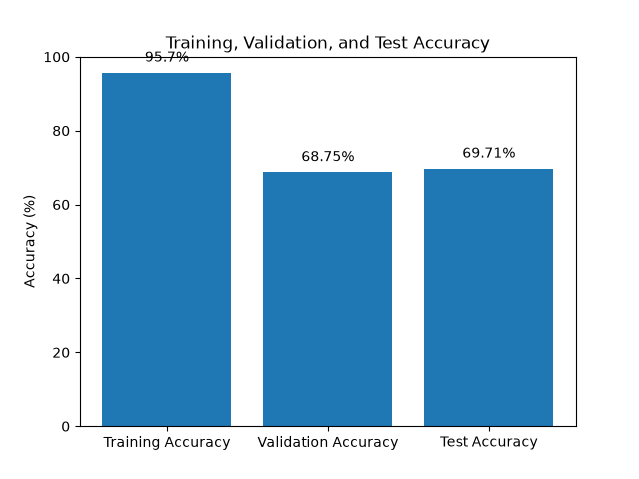
\includegraphics[width=1\linewidth]{mostrecentrunaccuracy.png}
    \caption{Training, Validation, and Test Accuracy}
    \label{fig:placeholder}
\end{figure}
\clearpage
\begin{figure}[h!]
    \centering
    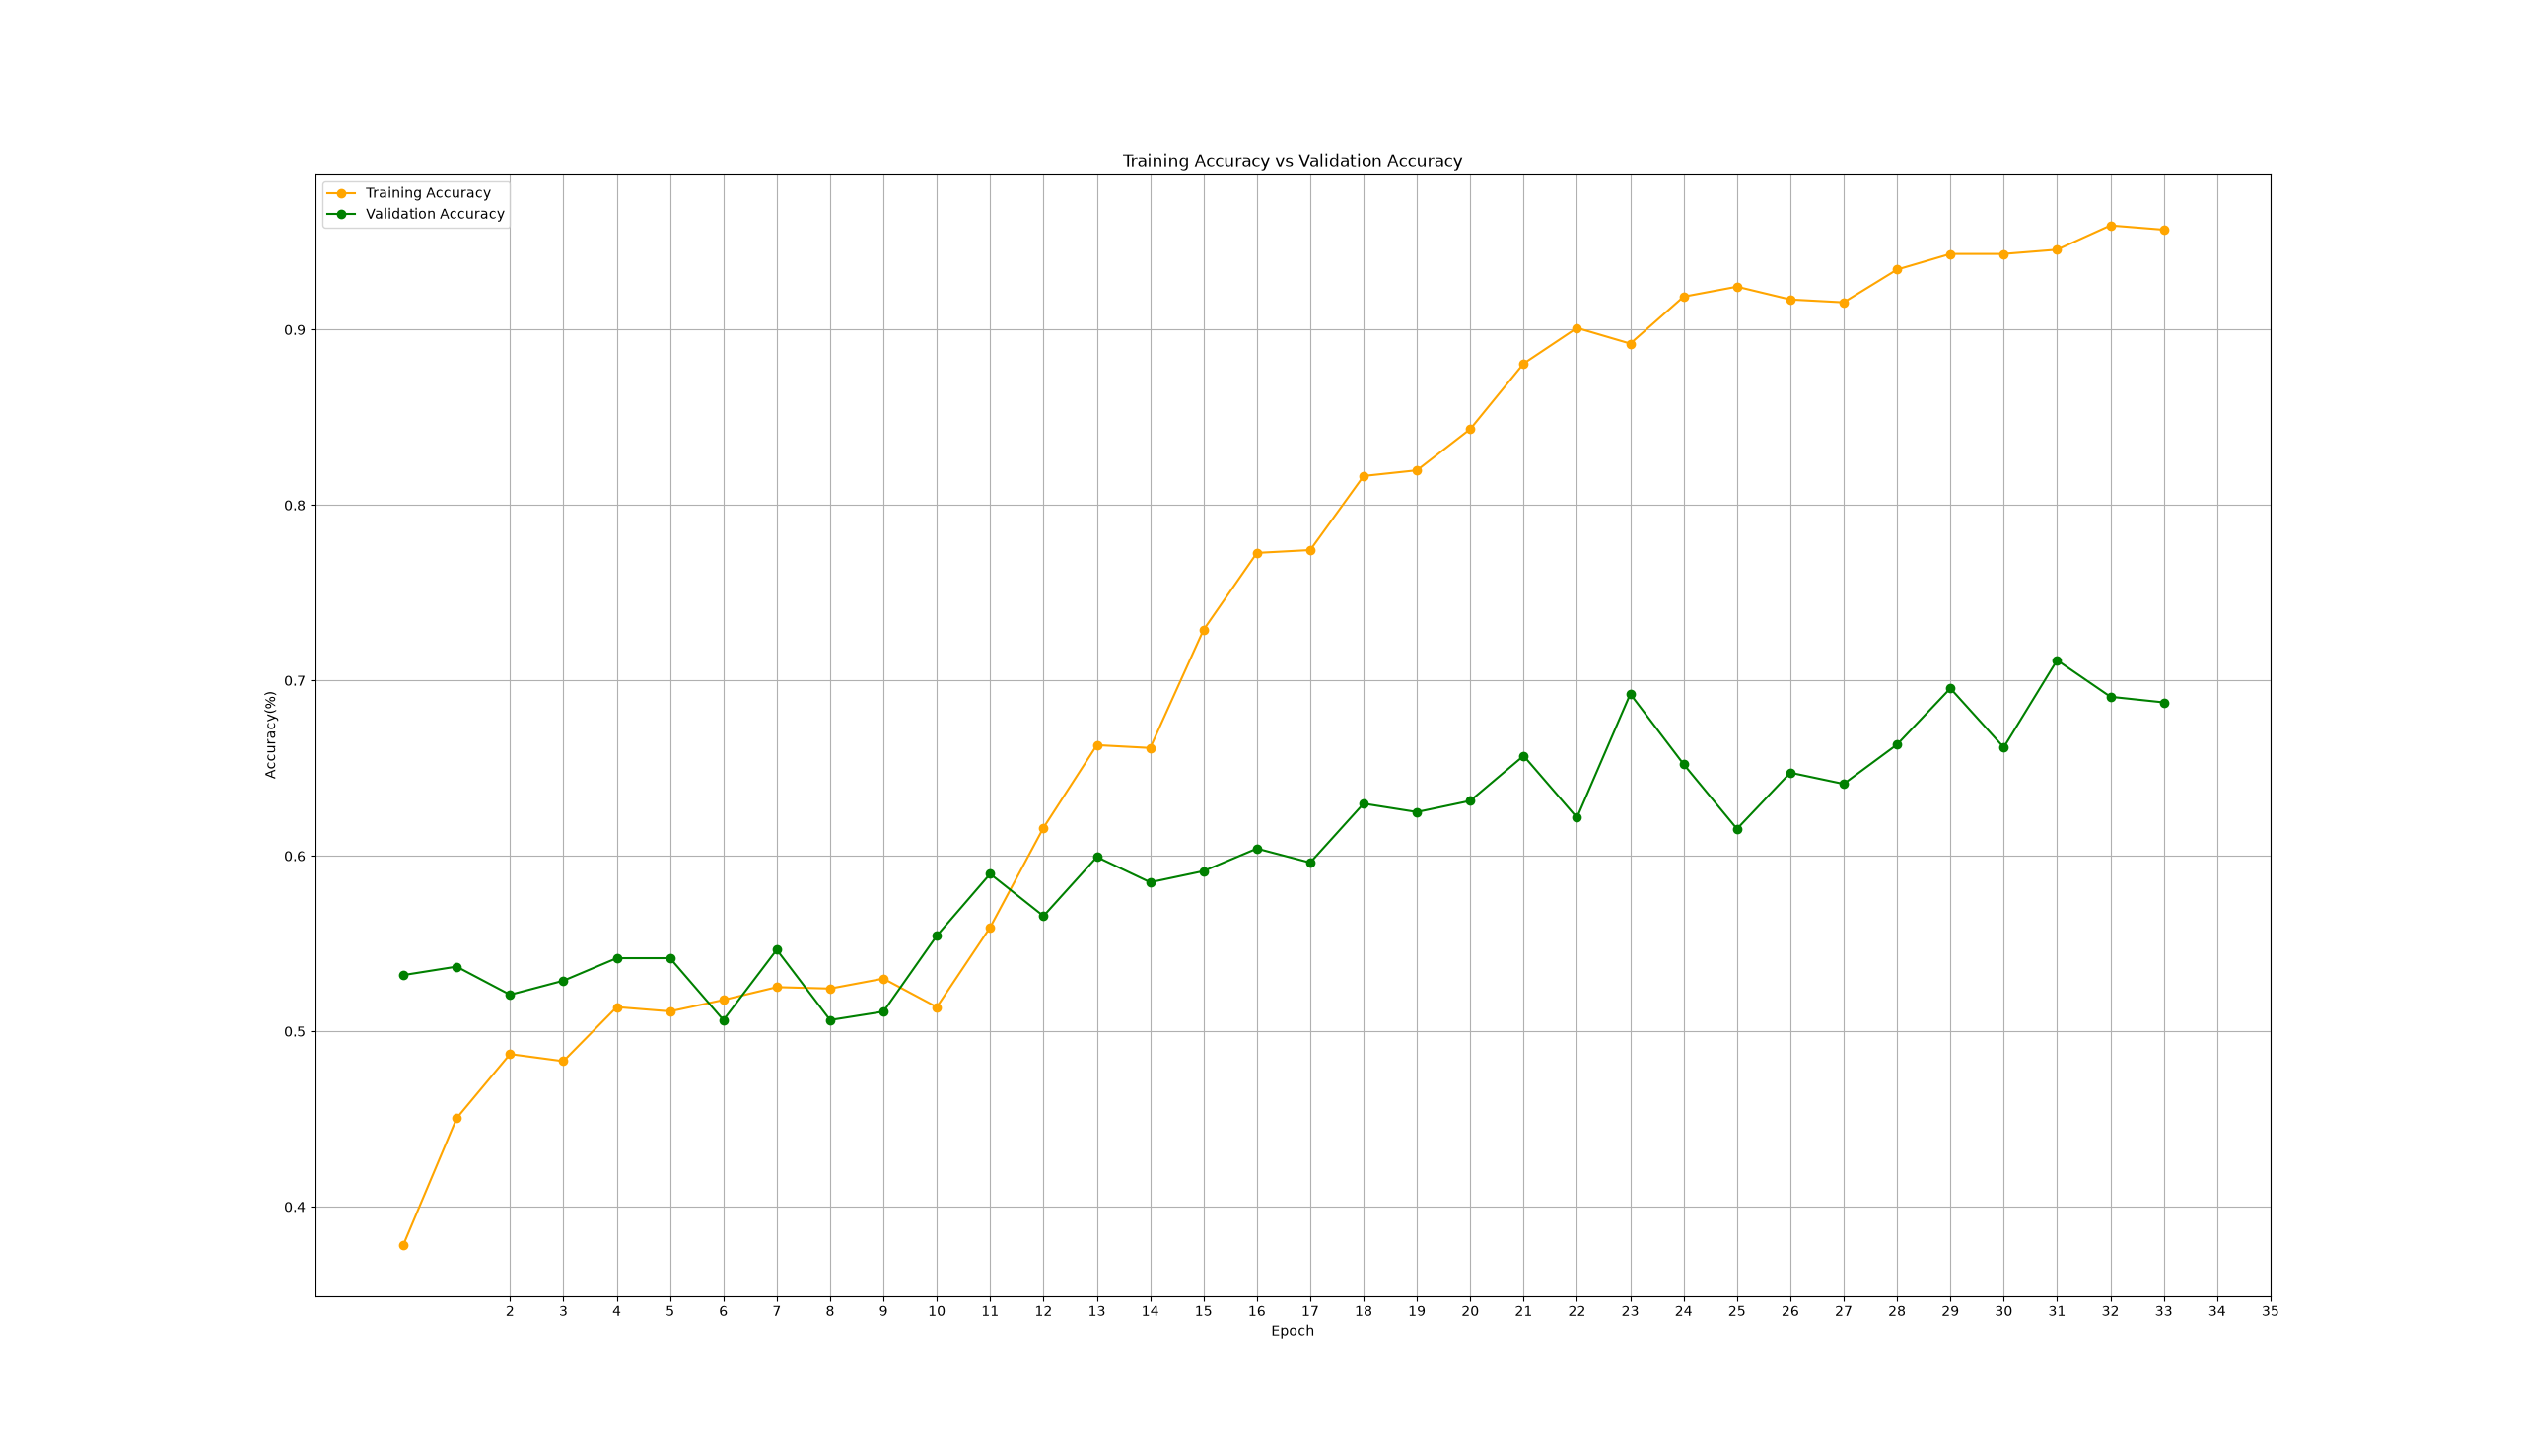
\includegraphics[width=1\linewidth]{mostrecentrunaccuracytrainval.png}
    \caption{Training and Validation Accuracy over Epochs}
    \label{fig:placeholder}
\end{figure}

\begin{figure}[h!]
    \centering
    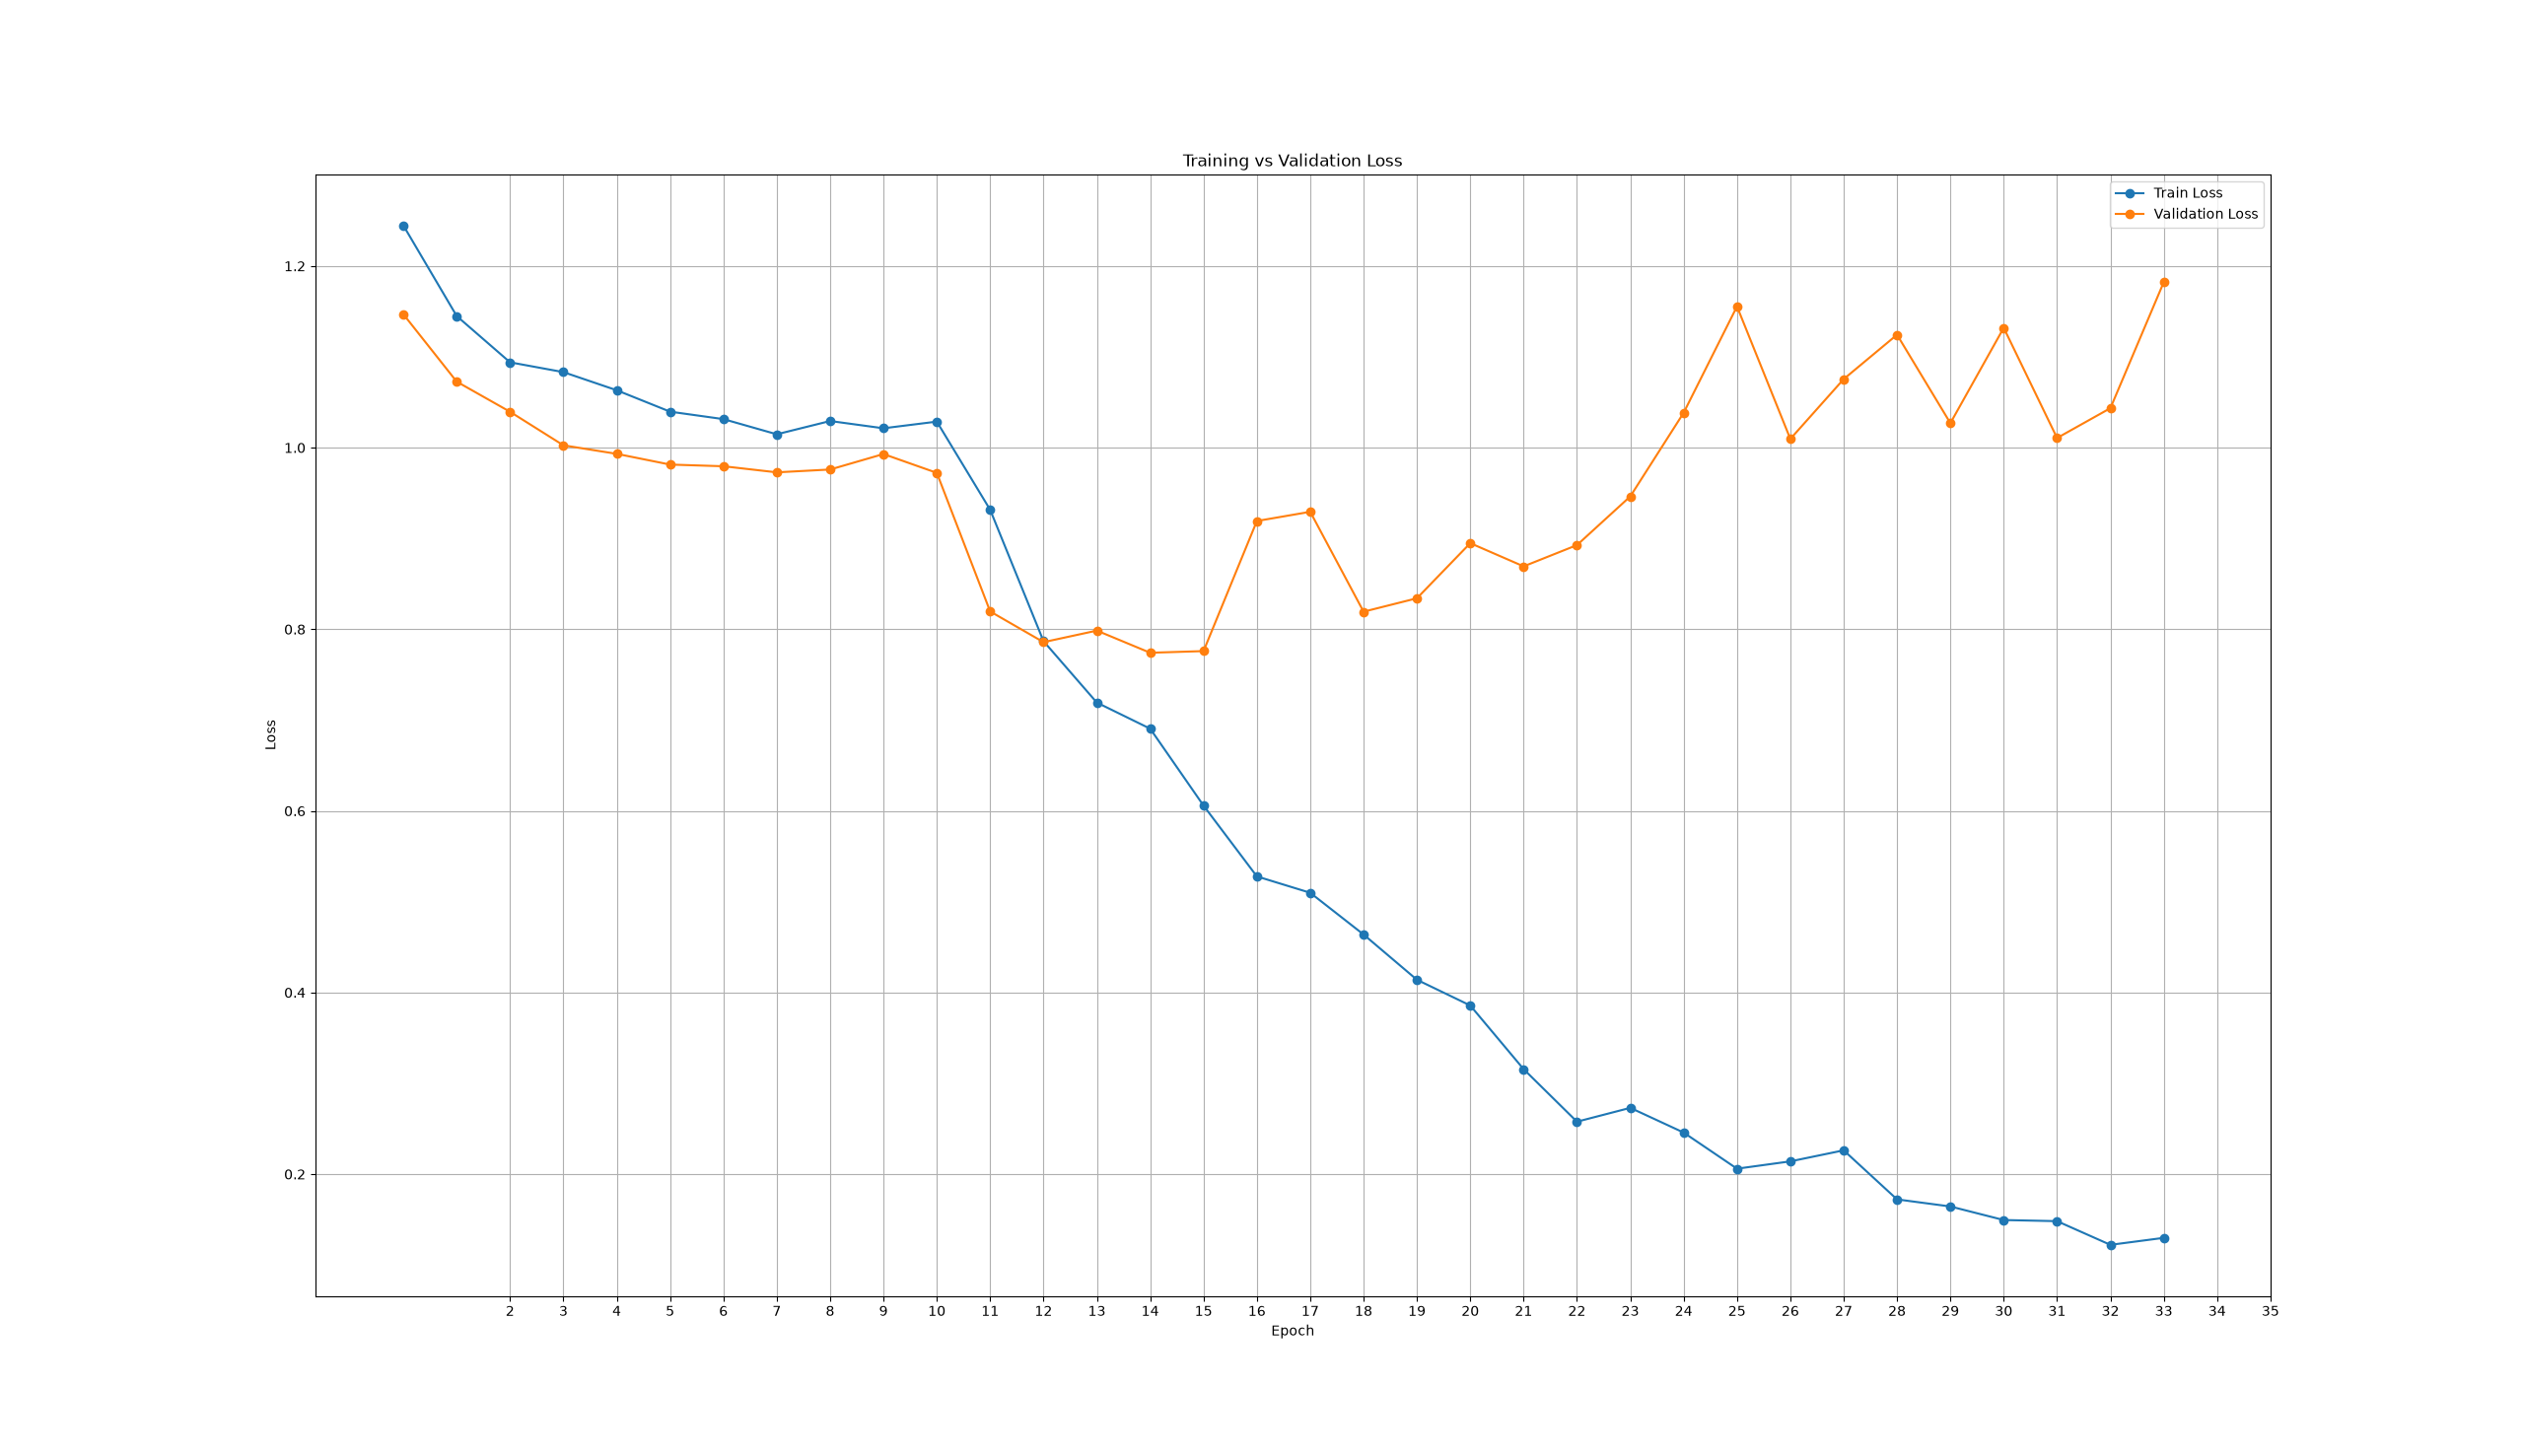
\includegraphics[width=1\linewidth]{mostrecentrunloss.png}
    \caption{Training and Validation Loss over Epochs}
    \label{fig:placeholder}
\end{figure}

\section{Conclusion}
The results show that this approach could be used to classify Rock Ptarmigan Sex and Age in the future if improved. The current test set accuracy of 69.71\% is significantly higher than random chance (25\%). However, the severe overfitting and relatively low accuracy of the model indicates that it will have to undergo significant improvements before it should be allowed to assist in classifying Rock Ptarmigans. 
Furthermore, this study has many limitations. First, this model was trained on a dataset of 3000 images, which is small for a classification problem with this much variance in between classes and likely contributed to the severe overfitting of the model. Additionally, the system this model is run on has 16 gigabytes of RAM memory, allowing training with smaller models such as EfficientNetB2 with small batch sizes of 16, but not for testing with larger models that require higher resolution images such as the EfficientNetB6 model.  
\section{Future Directions}
There are many different methods and directions this study could continue in to improve results. First and foremost, the model will have to go through more improvements and optimizations, specifically after the model backbone is unfrozen as that seems to be when overfitting occurs. Adding more regularization, harsher data augmentation, and reducing the inintial learning rate could help mitigate the amount of overfitting the current model is experiencing. Furthermore, more testing on other pretrained models as a base before applying transfer learning, such as OpenAI's CLIP \cite{DBLP:journals/corr/abs-2103-00020}, which was trained on a custom 400 million image dataset rather than the standard ImageNet dataset, could provide interesting results.

\section*{Acknowledgements}
I would like to thank my mentor Atul Ingle for his help and guidance throughout this project. I would also like to thank Doug Mandell, Karen Margolis, Mark Galassi, and the Institute for Computing in Research for making this opportunity possible.

\bibliographystyle{plain}
\bibliography{references}

\end{document}
